\documentclass[conference]{IEEEtran}
\usepackage{cite}
\usepackage{amsmath,amssymb,amsfonts}
\usepackage{graphicx}
\usepackage{booktabs}
\usepackage{multirow}
\usepackage{algorithm}
\usepackage{algpseudocode}
\usepackage{xcolor}
\usepackage{url}
\usepackage{CJKutf8}
\usepackage{tikz}
\usepackage[hidelinks]{hyperref}
\graphicspath{{figures/}}

\begin{document}

\title{An Explainable Tool-Augmented Agent for Short-Term Freeway Congestion Prediction and Departure Advisory: A Case Study on Taiwan National Freeway No.~5}

\author{\IEEEauthorblockN{First Author and Second Author}
\IEEEauthorblockA{Department of Computer Science and Engineering\\
National Chung Hsing University, Taichung, Taiwan\\
Email: jex1235@hotmail.com}}

\maketitle

\begin{abstract}
Severe holiday traffic congestion along Taiwan National Freeway No.~5---which connects Taipei and Yilan through the Hsuehshan Tunnel---poses persistent mobility challenges, with average daily freeway traffic volume during the 2026 Lunar New Year holiday reaching 124.0 million vehicle-kilometers (approximately $1.3\times$ the weekday annual average). Existing traffic forecasting models typically output isolated numerical speeds without regulatory context or explicit uncertainty boundaries, whereas emerging large language model (LLM) traffic assistants are prone to numerical hallucination and rarely ground responses in live roadside telemetry. Meanwhile, official mobility applications do not publish reproducible accuracy benchmarks. To bridge these gaps, this paper presents an explainable, tool-augmented congestion prediction and departure advisory agent designed under a ``prediction-as-a-tool, LLM-does-not-compute'' paradigm. Built on 5-minute electronic toll collection (ETC) gantry telemetry (TDCS M05A and \texttt{ETagPairLive.xml}) across 10 mainline segments of Freeway No.~5, the system integrates five modules: (1) domain data-aware preprocessing that filters zero-speed/zero-volume no-vehicle artifacts and enforces a verified $-3$-minute live-to-historical slot alignment; (2) histogram-based gradient boosting (\texttt{HistGradientBoosting}) models for $+15$/$+30$/$+60$-minute speed regression and isotonic-calibrated congestion risk estimation; (3) a 43-entry verified traffic-control knowledge base (high-occupancy vehicle rules and ramp closures) combined with live incident feeds; (4) a guardrailed agent enforcing deterministic numerical verification (\texttt{check\_numbers}) with safe template fallback; and (5) interactive CLI and Web interfaces. Trained on full-year 2024 data and evaluated on 2025 (365 days) and out-of-sample 2026 (311 days), the model achieves statistically significant speed MAE reductions over persistence on weekdays ($-0.39$ to $-0.75$~km/h in 2025; $-0.36$ to $-0.55$~km/h in 2026) and regular weekends ($-0.32$ to $-0.70$~km/h; $-0.31$ to $-0.50$~km/h), while gains on long holidays are smaller and year-dependent ($-0.04$~km/h, 95\% CI [$-0.17, +0.08$] at 60~min in 2026). Crucially, under a fixed-alert-budget event-level protocol (918 events in 2025; 680 in 2026), the deployed classifier does not outperform persistence for early congestion warning, demonstrating why risk scores must be distinguished from early-warning claims. Across 72 frozen agent evaluation cases (216 runs per mode), both LLM and template modes achieve 100\% deterministic guardrail compliance, with 86\% LLM adoption and zero numerical hallucinations.
\end{abstract}

\begin{IEEEkeywords}
Intelligent transportation systems, traffic congestion forecasting, explainable AI agent, tool-augmented large language models, probability calibration, Taiwan National Freeway No.~5.
\end{IEEEkeywords}

\section{Introduction}\label{sec:intro}

\subsection{Background and Motivation}
Electronic Toll Collection (ETC) gantry networks generate continuous, high-resolution roadside telemetry that supports real-time highway traffic monitoring and short-term forecasting. In Taiwan, National Freeway No.~5 (Chiang Wei-shui Memorial Freeway) serves as the primary arterial corridor linking the Taipei metropolitan area with Yilan County through the 12.9~km Hsuehshan Tunnel. Because the corridor has limited alternative routes and concentrated weekend and holiday travel demand, severe recurrent and holiday congestion frequently forms on northbound return approaches and tunnel bottlenecks. According to the Freeway Bureau, Ministry of Transportation and Communications (MOTC), average daily national freeway traffic during the 2026 Lunar New Year holiday (Days 1--6) reached 124.0 million vehicle-kilometers, approximately $1.3\times$ the weekday annual average of 93 million vehicle-kilometers~\cite{freeway2026cny}.

To assist travelers, official platforms such as the Freeway 1968 application provide real-time road conditions, travel-time forecasts, and departure-window recommendations. Concurrently, large language models (LLMs) have enabled conversational interfaces capable of translating complex system outputs into natural-language advisories. However, bridging roadside telemetry, predictive modeling, and actionable traveler communication in a transparent and verifiable workflow remains challenging.

\subsection{Problem Statement and Research Challenges}
Deploying a trustworthy short-term congestion advisory system on open roadside data exposes four practical gaps:
\begin{enumerate}
    \item \textbf{Isolated numerical outputs lack decision context:} Conventional forecasting models emit scalar speeds (e.g., 42~km/h) without linking predictions to active traffic-control regulations---such as High-Occupancy Vehicle (HOV) mandates or ramp closures---or live traffic incidents, nor do they communicate model limitations.
    \item \textbf{Domain data-quality pitfalls:} In Taiwan's open TDCS M05A 5-minute gantry dataset~\cite{tdcs_m05a}, intervals with zero passing vehicles are recorded with both \textit{speed = 0} and \textit{volume = 0}. Naive ingestion treats these records as severe standstill congestion (0~km/h), corrupting both training targets and congestion labels.
    \item \textbf{Numerical hallucination in LLM agents:} General-purpose LLMs are unreliable at quantitative forecasting and frequently fabricate or alter numerical values, omit mandatory caveats, or hallucinate unsupported road segments when left unconstrained.
    \item \textbf{Misleading evaluation protocols and opaque benchmarks:} Official services do not publish reproducible error metrics. In academic evaluations, sample-level F1 or ROC-AUC scores on imbalanced 5-minute series can appear deceptively high due to prolonged already-congested or free-flow regimes, masking poor early-warning performance when traffic is still free-flowing.
\end{enumerate}

\subsection{Main Contributions}
Rather than claiming superiority over official navigation apps or pursuing deep-learning leaderboard records, this study focuses on \textit{verifiable, explainable, and reproducible} decision support on Taiwan National Freeway No.~5 (10 mainline segments). Our main contributions are fourfold:
\begin{itemize}
    \item \textbf{Domain Data-Aware Ingestion and Live Alignment:} We establish deterministic preprocessing rules that distinguish no-vehicle records ($v=0, q=0$) from true congestion, bound forward-filling to 15~minutes, and empirically verify a $-3$-minute slot alignment between live \texttt{ETagPairLive.xml} and historical M05A archives (100\% match across 3,418 records).
    \item \textbf{``Prediction-as-a-Tool'' Guardrailed Agent Architecture:} All speed predictions, isotonic-calibrated risk probabilities, regulatory rule matches, and departure recommendations are computed deterministically by backend Python tools. The LLM (\texttt{qwen3-14b}) is restricted to query parsing and prose generation, protected by \texttt{check\_numbers} and \texttt{required\_missing} verification with automatic fallback to deterministic templates, plus programmatic post-appending of live incidents and holiday caveats.
    \item \textbf{Multi-Year Reproducible Evaluation with Fixed-Budget Event Analysis:} We evaluate a 2024-trained model across full-year 2025 (365 days) and out-of-sample 2026 (311 days) using day-level block bootstrap 95\% confidence intervals, latency degradation tests, and a fixed-alert-budget event-level early-warning protocol.
    \item \textbf{Transparent Reporting of Negative and Mixed Findings:} We explicitly document where machine learning helps (weekday and regular-weekend speed MAE) and where it does not (fragile holiday gains, early-warning parity with persistence, and high-probability calibration drift in 2026), reinforcing scientific rigor in applied ITS agents.
\end{itemize}

\subsection{Paper Organization}
Section~\ref{sec:related} reviews related work in traffic forecasting and LLM-based transportation agents. Section~\ref{sec:method} formulates the problem and details our five-module architecture and guardrailed algorithm. Section~\ref{sec:experiments} presents multi-year quantitative evaluations and end-to-end agent experiments. Section~\ref{sec:conclusion} concludes with system limitations and future research directions.

\section{Related Work}\label{sec:related}

\subsection{Short-Term Traffic Speed and Congestion Forecasting}
Short-term traffic forecasting methods span three major paradigms: classical statistical models, tabular machine learning, and deep spatiotemporal architectures. Classical approaches such as Historical Average (HA), ARIMA, and Support Vector Regression (SVR) offer transparent behavior and low computational overhead, making them essential baselines, but they struggle to capture non-linear congestion transitions under abrupt demand surges.

Deep spatiotemporal networks have achieved strong benchmark performance by modeling road networks as graphs. Diffusion Convolutional Recurrent Neural Networks (DCRNN)~\cite{li2018dcrnn} capture bidirectional spatial diffusion alongside recurrent temporal dynamics; Spatio-Temporal Graph Convolutional Networks (STGCN)~\cite{yu2018stgcn} replace recurrence with gated temporal convolutions for faster training; and Graph WaveNet~\cite{wu2019graphwavenet} introduces adaptive adjacency matrices and dilated causal convolutions. While effective on dense sensor benchmarks, these models act as opaque black boxes, require GPU infrastructure, and rarely report event-level early-warning accuracy under controlled alert budgets.

For structured tabular telemetry with moderate spatial dimensionality (such as a 10-segment corridor), histogram-based gradient boosted decision trees---popularized by LightGBM~\cite{ke2017lightgbm}---offer competitive accuracy, rapid CPU training, native handling of missing values and categorical segment identifiers, and straightforward reproducibility. Furthermore, raw classifier outputs in rare-event regimes are frequently miscalibrated~\cite{guo2017calibration}; non-parametric isotonic regression~\cite{zadrozny2002isotonic} provides a principled post-hoc calibration mechanism when fitted on held-out chronological splits.

\subsection{LLMs and Tool-Augmented Agents in Transportation}
Recent research has explored integrating LLMs into intelligent transportation systems (ITS) along two directions. First, foundation-model adaptations such as ST-LLM~\cite{liu2024stllm} and xTP-LLM~\cite{guo2024xtpllm} align spatiotemporal traffic embeddings with partially frozen LLMs to produce forecasts and textual explanations. Second, agentic frameworks inspired by ReAct~\cite{yao2023react}---notably TrafficGPT~\cite{zhang2024trafficgpt}---connect LLMs to external traffic simulation and analysis tools for interactive querying and decision support.

Despite their conversational flexibility, existing LLM traffic studies exhibit three recurring limitations for operational traveler advisories: (1) reliance on offline benchmark datasets or microscopic simulators rather than live open roadside feeds with real-world missingness and latency; (2) insufficient separation between numerical computation and text generation, leaving responses vulnerable to subtle numerical hallucination; and (3) omission of verified domain regulations (e.g., holiday HOV controls and ramp closures) and explicit scope-refusal boundaries.

\subsection{Research Gap and Positioning}
Table~\ref{tab:mae} and Section~\ref{sec:method} reflect how our system bridges these gaps: instead of asking an LLM to predict traffic directly or relying on an opaque black-box model alone, we pair lightweight tabular forecasting and isotonic calibration with a verified regulatory knowledge base, live incident feeds, and deterministic verification guardrails. Crucially, we evaluate both predictive utility (against persistence and historical average under strict chronological splits) and agent reliability (refusal accuracy, numerical fidelity, and fallback behavior).

\section{Proposed Scheme}\label{sec:method}

\subsection{Problem Formulation}
We model the mainline of Taiwan National Freeway No.~5 as a set of $K=10$ directed ETC gantry segments (5 southbound from 0.0K to 49.4K and 5 northbound from 52.8K to 0.1K), selected from mainline \texttt{05F} gantry pairs with $\ge 90\%$ valid training coverage. Time is discretized into 5-minute slots $t \in \{0, 1, \dots, 287\}$ per day. For segment $k$ at slot $t$, the roadside telemetry provides passenger-car (vehicle class 31) median speed $v_k(t)$ (km/h) and traffic volume $q_k(t)$.

We define a binary congestion indicator using a project-defined threshold $\tau = 40$~km/h:
\begin{equation}
c_k(t) = \mathbb{I}\!\left[v_k(t) < 40\right].
\label{eq:cong_ind}
\end{equation}
Given a query at decision time $T$ (slot $t$) for segment $k$ with historical observations up to $t$ and calendar metadata known prior to $T$, the prediction engine estimates multi-horizon future speed $\hat{v}_k(t+h)$ and calibrated congestion probability $\hat{p}_k(t+h)$ for horizons $h \in \{3, 6, 12\}$ slots ($+15, +30, +60$~minutes):
\begin{equation}
\hat{v}_k(t+h) = f_{\text{reg}}^{(h)}(\mathbf{x}_{k,t}), \qquad
\hat{p}_k(t+h) = g_{\text{cal}}^{(h, s_{k,t})}\!\left(f_{\text{clf}}^{(h)}(\mathbf{x}_{k,t})\right),
\label{eq:forecast}
\end{equation}
where $\mathbf{x}_{k,t} \in \mathbb{R}^{13}$ is the feature vector and $s_{k,t} \in \{0,1\}$ indicates whether the segment is currently in sustained free-flow ($v_k(t-j) \ge 40$ for all $j \in \{0,\dots,5\}$).

For event-level early-warning evaluation, a ground-truth \textit{congestion onset event} occurs at $(k, t^*)$ during 05:00--22:00 if $v_k(t^*) < 40$ while $v_k(t^*-j) \ge 40$ for all $j \in \{1,\dots,6\}$ (30 minutes of preceding free-flow).

\subsection{Five-Module System Architecture}
Fig.~\ref{fig:architecture} illustrates our five-module architecture built around the core principle that \textit{all numerical computations and safety rules reside in deterministic code, while the LLM only handles language parsing and prose rendering}.

\begin{figure*}[t]
\centering
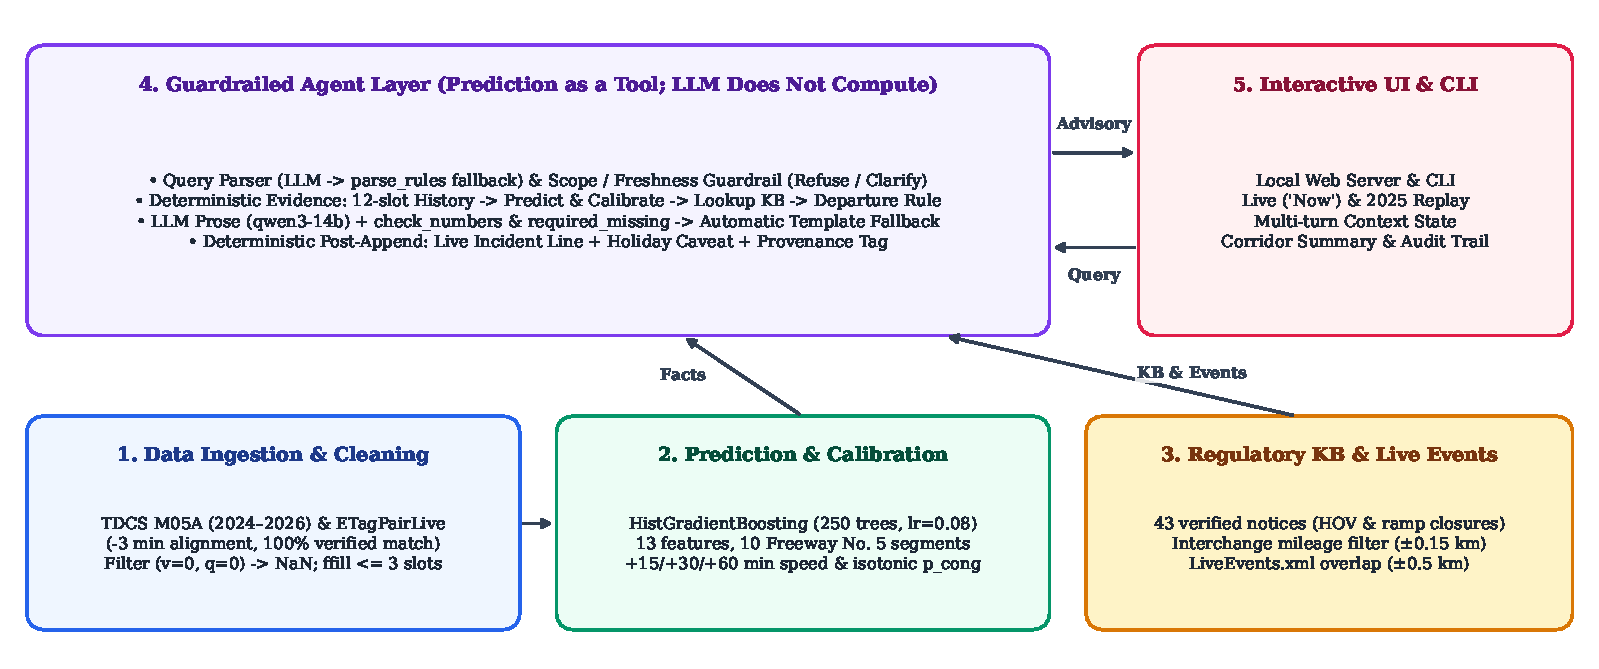
\includegraphics[width=0.95\textwidth]{architecture.pdf}
\caption{Five-module architecture of the explainable tool-augmented Freeway No.~5 congestion prediction agent. Numerical prediction, probability calibration, regulatory matching, and safety verification are executed deterministically outside the LLM.}
\label{fig:architecture}
\end{figure*}

\subsubsection{Module 1: Data Ingestion and Quality-Aware Preprocessing}
Historical archives from TDCS M05A (2024--2026) and live 5-minute XML feeds (\texttt{ETagPairLive.xml}) are normalized into unified daily arrays. Three domain data-quality safeguards are enforced:
\begin{itemize}
    \item \textbf{No-vehicle filtering:} Records with $v_k(t)=0$ and $q_k(t)=0$ (and outlier speeds $>150$~km/h) are converted to \texttt{NaN} rather than 0~km/h, preventing sensor inactivity or zero-flow periods from being mislabeled as extreme congestion.
    \item \textbf{Bounded imputation and cold-start guard:} Missing values are forward-filled up to at most 3 slots (15~min); if any required lag remains missing or $t < 60$ (before 05:00, where 1-hour history and training support are absent), the system refuses to forecast rather than extrapolating.
    \item \textbf{Exact live-to-historical alignment:} Comparing 3,418 passenger-car records on 2026-11-08 established 100\% speed and volume identity under the slot rule $\text{slot} = \lfloor (\text{update\_time} - 3\text{ min}) / 5\text{ min} \rfloor$, whereas unshifted or $-5$/$-8$/$-10$~min alignments yielded only 5\%--88\% agreement. In live mode, feeds older than 20~minutes trigger automatic refusal, and slots timestamped after current time \texttt{now} are excluded.
\end{itemize}

\subsubsection{Module 2: Prediction and Calibration Engine}
For each horizon $h \in \{15, 30, 60\}$~min, we train a scikit-learn \texttt{HistGradientBoostingRegressor} and \texttt{HistGradientBoostingClassifier} (250 boosting iterations, learning rate $0.08$), shared across all 10 segments with segment ID encoded as a categorical feature. Each sample uses 13 features: current speed $v_k(t)$, lagged speeds at $t-\{1,2,3,6,12\}$, 6-slot rolling mean and standard deviation, current volume $q_k(t)$, time-of-day slot, calendar day type (weekday, regular weekend, or long holiday $\ge 3$ consecutive days), holiday day-index (first/middle/final day), and segment ID. Day types are derived strictly from official 2024--2026 calendars so missing cache days never distort holiday classification.

Because raw classifier scores exhibited severe overconfidence during free-flow periods (predicting $\ge 0.9$ on 182 instances with 0 actual congestions), we fit group-wise isotonic regression calibrators~\cite{zadrozny2002isotonic} on held-out 2025 H1 data, stratified by $s_{k,t}$ (currently free-flow vs.\ otherwise) and horizon $h$.

\subsubsection{Module 3: Verified Regulatory Knowledge Base and Live Incidents}
We maintain a structured JSON knowledge base (\texttt{announcements.json}) containing 43 verified traffic-control announcements across 2024 (3), 2025 (20), and 2026 (20), covering HOV restrictions (e.g., 13:00--18:00 northbound at Suao, Luodong, Yilan, and Toucheng ramps) and southbound ramp closures (Shiding and Pinglin). Each record stores applicable dates, road, direction, active time window, verbatim text, source URL, and provenance level (\textit{official notice} vs.\ \textit{media relay}). Announcements are matched to queried segments via interchange mileage with $\pm 0.15$~km tolerance, distinguishing \textit{active} vs.\ \textit{starting within 60~min} rules. In live mode, \texttt{LiveEvents.xml} is parsed to attach direction-matched Freeway No.~5 incidents overlapping the segment ($\pm 0.5$~km). Because neither regulations nor incidents enter the ML feature matrix, they are explicitly presented alongside predictions with clear disclosure.

\subsubsection{Module 4: Guardrailed Agent Layer}
The agent follows a deterministic pipeline (\texttt{Understand} $\rightarrow$ \texttt{Plan} $\rightarrow$ \texttt{Acquire} $\rightarrow$ \texttt{Analyze} $\rightarrow$ \texttt{Lookup} $\rightarrow$ \texttt{Compose}), detailed in Algorithm~\ref{alg:agent}. An OpenAI-compatible local LLM (\texttt{qwen/qwen3-14b} via LM Studio) is used only in two bounded places: (1) extracting structured slots (road, origin, destination, time) from user queries, with automatic fallback to deterministic regular-expression parsing (\texttt{parse\_rules}) while date, direction, and out-of-scope intent are always resolved in code; and (2) composing concise natural-language advice from a serialized \texttt{facts\_text} bundle.

To eliminate numerical hallucination, every LLM response must pass two deterministic validators:
\begin{itemize}
    \item \texttt{check\_numbers}: Every numeric token in the generated text must appear in \texttt{facts\_text} (with standard horizon constants 15, 30, 60 permitted).
    \item \texttt{required\_missing}: The response must retain the rule-selected waiting interval and any active announcement time window.
\end{itemize}
If either check fails or the LLM endpoint is unreachable, the agent transparently falls back to a deterministic template. Finally, live incident lines and holiday accuracy caveats are appended programmatically \textit{after} LLM generation (prompted by empirical testing showing that the LLM omitted holiday caveats in 60\% of holiday queries when left unguarded).

\subsubsection{Module 5: Interactive Presentation}
Both a local Web UI (\texttt{server.py}) and CLI (\texttt{ask.py}) support live (``now'') queries, 2025 historical replay, multi-turn context carryover (date, time, direction, origin), and corridor-wide summary tables, always tagging each response with its provenance (\texttt{[LLM]} or \texttt{[Template: reason]}).

\subsection{Core Advisory Algorithm}
Algorithm~\ref{alg:agent} formalizes the end-to-end decision and verification logic. Candidate departure times $\Delta \in \{0, 15, 30, 60\}$~min are ranked deterministically by minimizing calibrated congestion probability rounded to $0.1$ (ties broken by earliest departure): if $\max_h \hat{p}_k(t+h) < 0.3$, the agent advises departing now; if the minimum candidate risk is $\ge 0.6$, it warns that no smooth window exists within 60~min; otherwise it recommends departing at $\Delta^*$.

\begin{algorithm}[t]
\caption{Guardrailed Congestion Prediction and Advisory Pipeline}
\label{alg:agent}
\begin{algorithmic}[1]
\Require User query $Q$, conversation state $S$, mode $m \in \{\text{live}, \text{replay}\}$
\Ensure Verified advisory response $R$ with provenance tag
\State $P \gets \text{ParseQuery}(Q, S)$ \Comment{LLM extractor; fallback \texttt{parse\_rules}}
\State Resolve date, direction, and intent deterministically from $Q, S$
\If{road $\neq$ Freeway~5 \textbf{or} unsupported intent/year}
    \State \Return $\text{RefuseWithScope}(P)$
\ElsIf{missing required date, time, or direction}
    \State \Return $\text{ClarifyMissing}(P)$
\EndIf
\If{$m = \text{live}$ \textbf{and} ($\text{age} > 20\text{ min}$ \textbf{or} $\text{time} < \text{05:00}$)}
    \State \Return $\text{RefuseDataUnavailable}()$
\EndIf
\State $\mathbf{H} \gets \text{GetRecent}(k, t, 12)$ \Comment{Quality-cleaned 60-min history}
\State $\mathbf{X} \gets \text{BuildFeatures}(\mathbf{H}, \text{calendar\_day\_type}(T))$
\If{$\mathbf{X}$ invalid (insufficient data)}
    \State \Return $\text{ReportInsufficientData}()$
\EndIf
\State $\{\hat{v}_k(t+h), \hat{p}_k(t+h)\}_{h \in \{15,30,60\}} \gets \text{PredictAndCalibrate}(\mathbf{X})$
\State $\mathcal{A} \gets \text{LookupKB}(\text{road}, \text{dir}, T, \text{seg\_km} \pm 0.15)$
\State $d^* \gets \text{SelectDepartureRule}(\{\hat{p}_k(t+h)\})$
\State $F \gets \text{SerializeFacts}(\hat{v}, \hat{p}, \mathcal{A}, d^*, \text{limitations})$
\State $R_{\text{raw}} \gets \text{ComposeLLM}(F)$
\If{\textbf{not} $\text{CheckNumbers}(R_{\text{raw}}, F)$ \textbf{or} $\text{RequiredMissing}(R_{\text{raw}}, d^*, \mathcal{A})$}
    \State $R_{\text{core}} \gets \text{ComposeTemplate}(F)$ \Comment{Deterministic fallback}
\Else
    \State $R_{\text{core}} \gets R_{\text{raw}}$
\EndIf
\State $R \gets \text{AppendFixed}(R_{\text{core}}, \text{Events}, \text{HolidayNote}, \text{Tag})$
\State \Return $R$
\end{algorithmic}
\end{algorithm}

\section{Experimental Results and Discussion}\label{sec:experiments}

\subsection{Experimental Setup and Baselines}
All predictive models are trained strictly on full-year 2024 TDCS M05A telemetry across the 10 Freeway No.~5 mainline segments. Evaluation is performed chronologically on two unseen periods: (1) the full 2025 test year (365 days: 247 weekdays, 87 regular weekends, 31 long-holiday days) and (2) an out-of-sample 2026 period from January~1 to November~8, 2026 (311 days: 206 weekdays, 73 regular weekends, 32 long-holiday days). Probability calibrators are fitted on 2025~H1 and evaluated on 2025~H2 and 2026.

We compare our \texttt{HistGradientBoosting} model (GBM) against two strong, transparent baselines:
\begin{itemize}
    \item \textbf{Persistence:} Predicts $\hat{v}_k(t+h) = v_k(t)$ (current speed persists). Any short-term model must first beat persistence.
    \item \textbf{Historical Average (HA):} Lookup mean speed by segment, time-of-day slot, and calendar day type computed on 2024 training data (no real-time input).
\end{itemize}
Because 5-minute samples within the same day are strongly autocorrelated, all 95\% confidence intervals (CIs) are computed via day-level block bootstrap with paired differences between methods. Software reproducibility is backed by 40 unit tests (\texttt{pytest}) covering alignment, stale-data refusal, rule parsing, knowledge-base filtering, and numerical verification.

\subsection{Speed Prediction Accuracy}
Table~\ref{tab:mae} and Fig.~\ref{fig:mae} report speed Mean Absolute Error (MAE, in km/h) stratified by horizon and day type across 2025 and 2026. Three findings emerge:
\begin{enumerate}
    \item \textbf{Consistent gains on weekdays and regular weekends:} Across all three horizons and both years, GBM significantly outperforms both HA and Persistence. At the 60-minute horizon, weekday MAE drops from 3.77 to 3.02~km/h ($\Delta = -0.75$, 95\% CI [$-0.79, -0.70$]) in 2025 and from 3.66 to 3.11~km/h ($\Delta = -0.55$, [$-0.60, -0.50$]) in 2026. Regular-weekend 60-minute MAE improves by $-0.70$~km/h in 2025 and $-0.50$~km/h in 2026. HA performs poorly on weekends ($>8$~km/h) and holidays ($>9.8$~km/h) because it ignores live traffic states.
    \item \textbf{Fragile and small gains on long holidays:} Holiday improvements over persistence are substantially smaller and unstable across years. At 60~minutes, GBM reduces holiday MAE by $-0.31$~km/h ([$-0.41, -0.20$]) in 2025, but in 2026 the difference shrinks to $-0.04$~km/h with a 95\% CI of [$-0.17, +0.08$] spanning zero.
    \item \textbf{Modest absolute magnitude:} Even when statistically significant, absolute reductions over persistence range from $0.04$ to $0.75$~km/h relative to base MAEs of $2.5$--$4.9$~km/h. Consequently, any claim of forecasting superiority must be reported by day type, and our agent explicitly appends a holiday accuracy caveat whenever the queried date falls on a long holiday.
\end{enumerate}

\begin{table*}[t]
\caption{Speed Prediction MAE (km/h) and Paired Difference Against Persistence (GBM $-$ Persistence) with Day-Level Bootstrap 95\% Confidence Intervals}
\label{tab:mae}
\centering
\begin{tabular}{llcccccccc}
\toprule
\multirow{2}{*}{Horizon} & \multirow{2}{*}{Day Type} & \multicolumn{4}{c}{2025 Test Year (365 Days)} & \multicolumn{4}{c}{2026 Out-of-Sample (311 Days)} \\
\cmidrule(lr){3-6} \cmidrule(lr){7-10}
 & & HA & Persist. & GBM & $\Delta$ (95\% CI) & HA & Persist. & GBM & $\Delta$ (95\% CI) \\
\midrule
\multirow{3}{*}{15 min}
 & Weekday     & 4.18 & 2.60 & \textbf{2.22} & $-0.39$ [$-0.40, -0.38$] & 4.68 & 2.56 & \textbf{2.20} & $-0.36$ [$-0.38, -0.35$] \\
 & Weekend     & 8.12 & 2.84 & \textbf{2.51} & $-0.32$ [$-0.34, -0.30$] & 8.54 & 2.79 & \textbf{2.48} & $-0.31$ [$-0.34, -0.28$] \\
 & Holiday     & 9.87 & 2.72 & \textbf{2.53} & $-0.19$ [$-0.23, -0.15$] & 10.50 & 2.61 & \textbf{2.47} & $-0.14$ [$-0.18, -0.10$] \\
\midrule
\multirow{3}{*}{30 min}
 & Weekday     & 4.19 & 3.03 & \textbf{2.56} & $-0.47$ [$-0.49, -0.46$] & 4.70 & 2.96 & \textbf{2.56} & $-0.40$ [$-0.43, -0.38$] \\
 & Weekend     & 8.20 & 3.59 & \textbf{3.20} & $-0.40$ [$-0.45, -0.35$] & 8.61 & 3.50 & \textbf{3.16} & $-0.34$ [$-0.39, -0.29$] \\
 & Holiday     & 9.97 & 3.37 & \textbf{3.19} & $-0.18$ [$-0.23, -0.14$] & 10.59 & 3.23 & \textbf{3.17} & $-0.06$ [$-0.11, -0.01$] \\
\midrule
\multirow{3}{*}{60 min}
 & Weekday     & 4.22 & 3.77 & \textbf{3.02} & $-0.75$ [$-0.79, -0.70$] & 4.74 & 3.66 & \textbf{3.11} & $-0.55$ [$-0.60, -0.50$] \\
 & Weekend     & 8.35 & 4.85 & \textbf{4.15} & $-0.70$ [$-0.81, -0.58$] & 8.77 & 4.71 & \textbf{4.21} & $-0.50$ [$-0.62, -0.38$] \\
 & Holiday     & 10.15 & 4.44 & \textbf{4.13} & $-0.31$ [$-0.41, -0.20$] & 10.78 & 4.28 & 4.24 & $-0.04$ [$-0.17, +0.08$] \\
\bottomrule
\end{tabular}
\end{table*}


\begin{figure*}[t]
\centering
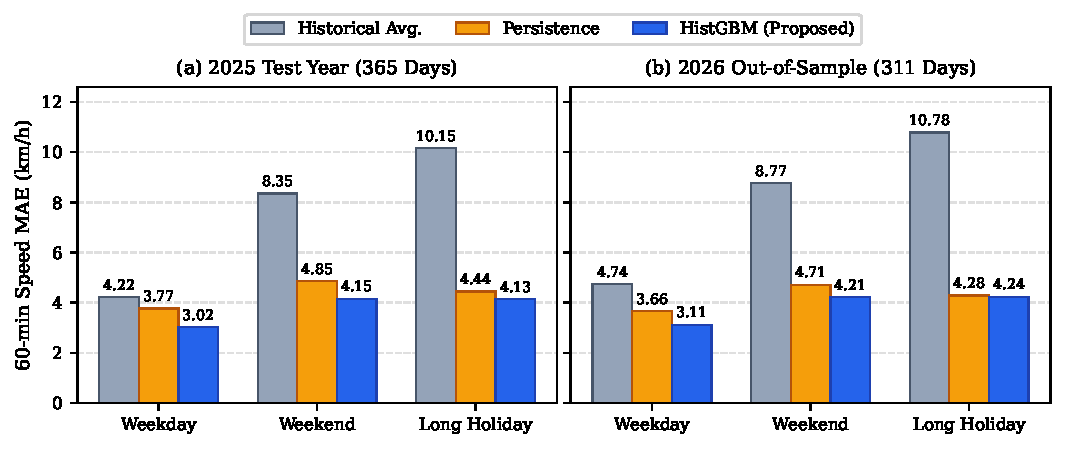
\includegraphics[width=0.92\textwidth]{mae_comparison.pdf}
\caption{Comparison of 60-minute speed prediction MAE (km/h) across day types for (a) the 2025 test year and (b) the 2026 out-of-sample period. While HistGBM consistently beats Persistence on weekdays and weekends, holiday gains are marginal in 2025 and statistically indistinguishable from zero in 2026.}
\label{fig:mae}
\end{figure*}

\subsection{Event-Level Early-Warning Evaluation}
Although sample-level congestion ROC-AUC appears very high (in 2026 out-of-sample data across $>637{,}000$ slots: 0.997 at 15~min, 0.993 at 30~min, and 0.986 at 60~min with only $\approx 2.6\%$ positive rate), sample-level metrics are dominated by prolonged already-congested or free-flow regimes and cannot measure \textit{advance warning}.

We therefore evaluate true early warning under a strict event-level protocol: alerts are evaluated \textit{only} when traffic is currently free-flowing ($v_k \ge 40$~km/h over the last 30~min); consecutive alerts on the same segment within 30~min are merged; thresholds are matched to fixed alert budgets of $0.25$, $0.50$, and $1.00$ alerts/segment/day; and an event is counted as detected if an alert fires within 60~min before onset (precision counts alerts followed by an event within 60~min).

Table~\ref{tab:events} and Fig.~\ref{fig:events} reveal a critical negative finding:
\begin{itemize}
    \item \textbf{Deployed classifier underperforms persistence:} At the low-noise 0.25 alert budget, the deployed classifier achieves only 0.42 detection (0.42 precision) in 2025 and 0.26 detection (0.23 precision) in 2026, trailing simple Persistence (0.70 / 0.73 in 2025; 0.76 / 0.71 in 2026) with non-overlapping CIs.
    \item \textbf{Dedicated onset model fails pre-registered deployment gate:} We trained a specialized \texttt{Onset} classifier exclusively on free-flow samples using speed-trend, recent-minimum, and volume-change features. While it closed the gap and slightly beat Persistence at the 0.50 budget ($+0.038$ [$+0.023, +0.053$] in 2025; $+0.031$ [$+0.018, +0.045$] in 2026), it failed our pre-registered success criterion requiring the 95\% CI lower bound to exceed zero at \textit{both} 0.25 and 0.50 budgets in 2025 (at 0.25: $+0.032$ [$-0.004, +0.070$]; on 2026 holidays at 0.50: $+0.000$ [$-0.047, +0.052$]). Adhering to our pre-registered gate, we did \textit{not} integrate the Onset model into the agent and explicitly frame calibrated probabilities as relative risk indicators rather than early-warning alarms.
\end{itemize}

\begin{table}[t]
\caption{Event-Level Early-Warning Detection Rate / Precision Under Fixed Alert Budgets (Alerts per Segment per Day)}
\label{tab:events}
\centering
\setlength{\tabcolsep}{4pt}
\begin{tabular}{llccc}
\toprule
Period & Method & 0.25 & 0.50 & 1.00 \\
\midrule
\multirow{4}{*}{\shortstack[l]{2025 Full\\(918 events)}}
 & Persistence & 0.70 / 0.73 & 0.91 / 0.48 & 0.96 / 0.26 \\
 & Hist. Avg.  & 0.36 / 0.37 & 0.61 / 0.32 & 0.97 / 0.25 \\
 & Deployed Clf. & 0.42 / 0.42 & 0.84 / 0.43 & 0.97 / 0.25 \\
 & Onset Model$^{\dagger}$ & \textbf{0.73 / 0.75} & \textbf{0.95 / 0.48} & \textbf{0.97 / 0.25} \\
\midrule
\multirow{4}{*}{\shortstack[l]{2026 Full\\(680 events)}}
 & Persistence & 0.76 / 0.71 & 0.94 / 0.43 & 0.96 / 0.22 \\
 & Hist. Avg.  & 0.34 / 0.39 & 0.65 / 0.29 & 0.99 / 0.22 \\
 & Deployed Clf. & 0.26 / 0.23 & 0.83 / 0.37 & 0.98 / 0.22 \\
 & Onset Model$^{\dagger}$ & \textbf{0.79 / 0.70} & \textbf{0.97 / 0.43} & \textbf{0.98 / 0.22} \\
\bottomrule
\multicolumn{5}{l}{\footnotesize $^{\dagger}$Not integrated into Agent: failed pre-registered 0.25-budget CI criterion.}
\end{tabular}
\end{table}


\begin{figure}[t]
\centering
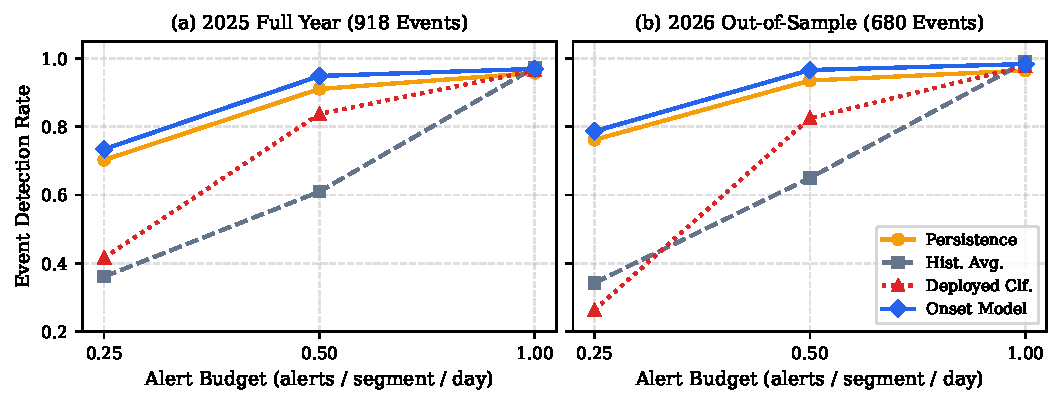
\includegraphics[width=\columnwidth]{event_warning.pdf}
\caption{Event-level early-warning detection rate under fixed alert budgets (0.25, 0.50, 1.00 alerts/segment/day) for (a) 2025 and (b) 2026. The deployed classifier trails Persistence at low alert budgets, illustrating the pitfalls of relying on sample-level AUC.}
\label{fig:events}
\end{figure}

\subsection{Probability Calibration and Data Latency Robustness}
On 2025~H2 free-flow samples with predicted congestion risk $\ge 0.3$, grouped isotonic calibration reduced the absolute gap between mean predicted probability and observed congestion frequency from $0.263 \rightarrow 0.082$ (15~min), $0.165 \rightarrow 0.042$ (30~min), and $0.034 \rightarrow 0.028$ (60~min), satisfying our pre-registered target ($\le 0.10$ across all horizons). However, on out-of-sample 2026 data (where positives cluster on fewer days), calibrated high-risk bins remained overestimated by roughly $2\times$ (e.g., 30-min mean predicted $0.45$ vs.\ observed $0.24$), confirming that probabilities should be communicated as qualitative risk levels rather than exact frequencies.

To assess operational resilience under feed delays, we simulated decision-time telemetry lags of $0, 5, 10,$ and $15$~minutes on 2025 data without retraining. At the 60-minute horizon, GBM MAE increased gradually from $3.39$ to $3.59$~km/h (approximately $+0.1$~km/h per 5-minute delay), whereas Persistence degraded from $4.09$ to $4.49$~km/h; thus, a 15-minute-delayed GBM still outperformed zero-delay Persistence.

\subsection{End-to-End Agent Evaluation}
We evaluated the complete agent across 72 frozen test cases (60 core cases covering normal queries, out-of-scope refusals, missing-slot clarifications, directional inference, announcement matching, missing data, and tool failures, plus 12 live-mode, open-phrasing, and holiday-caveat cases), executed 3 times per case in both Template and LLM (\texttt{qwen/qwen3-14b}) modes. Results are summarized in Table~\ref{tab:agent}.

Both modes achieved 100\% across all deterministic guardrail checks, including zero numerical hallucinations, exact announcement citations, and 3-run consistency. In LLM mode, approximately 86\% of responses were accepted directly, while the remaining 14\% triggered safe fallback to the deterministic template due to numerical or required-content verification failures. Median latency was $\approx 2$~s in Template mode and $9$--$14$~s (p95: $20$--$24$~s) in LLM mode.

Critically, we caution against over-interpreting these 100\% automated scores: because test phrasings mirror rule patterns and core decisions are deterministic, automated metrics verify regression safety rather than natural-language quality under unconstrained user queries. Indeed, prior to adding programmatic post-appending, the LLM voluntarily included the holiday caveat in only 40\% (31/78) of holiday runs---a defect invisible until explicitly encoded into both deterministic post-processing and scoring rubrics. Formal human evaluation of readability and helpfulness remains future work.

\begin{table}[t]
\caption{End-to-End Agent Evaluation Across 72 Frozen Cases (3 Runs Each, Total 216 Executions per Mode)}
\label{tab:agent}
\centering
\begin{tabular}{lcc}
\toprule
Metric & Template Mode & LLM Mode (\texttt{qwen3-14b}) \\
\midrule
Refusal \& Clarification Accuracy & 100\% & 100\% \\
Zero Numerical Hallucination & 100\% & 100\% \\
Announcement Citation Accuracy & 100\% & 100\% \\
Advisory-Rule Consistency & 100\% & 100\% \\
Holiday Caveat Inclusion & 100\% & 100\%$^{\ddagger}$ \\
3-Run Consistency & 100\% & 100\% \\
LLM Output Adoption Rate & --- & $\approx$86\% (14\% fallback) \\
Median Latency (p50) & $\approx$2 s & 9--14 s (p95: 20--24 s) \\
\bottomrule
\multicolumn{3}{l}{\footnotesize $^{\ddagger}$40\% (31/78) when left to LLM; 100\% after deterministic post-append.}
\end{tabular}
\end{table}


\section{Conclusion and Future Work}\label{sec:conclusion}

This paper presented an explainable, tool-augmented agent for short-term congestion prediction and departure advisory on Taiwan National Freeway No.~5. By enforcing a strict division of labor---where domain-cleaned ETC gantry telemetry, \texttt{HistGradientBoosting} regressors, isotonic probability calibrators, a 43-entry verified traffic-control knowledge base, and live incident feeds supply deterministic facts, while the LLM focuses solely on query parsing and natural-language rendering under \texttt{check\_numbers} and template-fallback guardrails---the system eliminates numerical hallucination while remaining fully operational even without an active LLM endpoint.

Multi-year evaluation across 2025 (365 days) and out-of-sample 2026 (311 days) demonstrates consistent speed MAE improvements over persistence on weekdays and regular weekends, graceful degradation under up to 15~minutes of telemetry latency, and 100\% deterministic guardrail compliance across 72 frozen agent test cases. Equally important, our rigorous evaluation exposes critical operational boundaries: long-holiday speed gains are modest and year-dependent; the deployed classifier does not beat persistence for event-level early warning under fixed alert budgets; and calibrated probabilities still exhibit overconfidence in rare high-risk bins across years.

\subsection{Limitations and Future Work}
Several limitations define clear priorities for future research:
\begin{enumerate}
    \item \textbf{Modeling and external signals:} Our study evaluated a shared tabular GBM without benchmarking against deep spatiotemporal architectures (e.g., Graph WaveNet or ST-Transformer) and without incorporating weather, non-recurrent accident records, or scheduled local events. Integrating multimodal features and periodic retraining pipelines may improve holiday robustness.
    \item \textbf{Advisory outcome validation and human evaluation:} The departure-window rule minimizes rounded calibrated congestion risk, but its actual reduction in traveler journey time has not yet been empirically validated. Likewise, systematic human evaluation on free-form queries is needed to quantify the communicative benefit of LLM prose over deterministic templates.
    \item \textbf{Knowledge-base and scope extensions:} Future iterations should incorporate announcement publication timestamps to prevent temporal leakage in historical replays, support vehicle-type and occupancy-exemption clarifications for HOV enforcement, verify gantry-code-to-mileage mappings against official specifications, and expand corridor coverage beyond Freeway No.~5.
\end{enumerate}


\section*{Acknowledgment}
Traffic telemetry data (TDCS M05A, \texttt{ETagPairLive.xml}, and \texttt{LiveEvents.xml}) are provided by the Freeway Bureau, Ministry of Transportation and Communications (MOTC), Taiwan, under the Taiwan Open Government Data License, Version~1.0. Calendar data are derived from the Taiwan Open Government Data Platform (Directorate-General of Personnel Administration) via \texttt{ruyut/TaiwanCalendar} under CC~BY~4.0.

\bibliographystyle{IEEEtran}
\bibliography{references}

\newpage
\vspace*{\fill}
\begin{center}
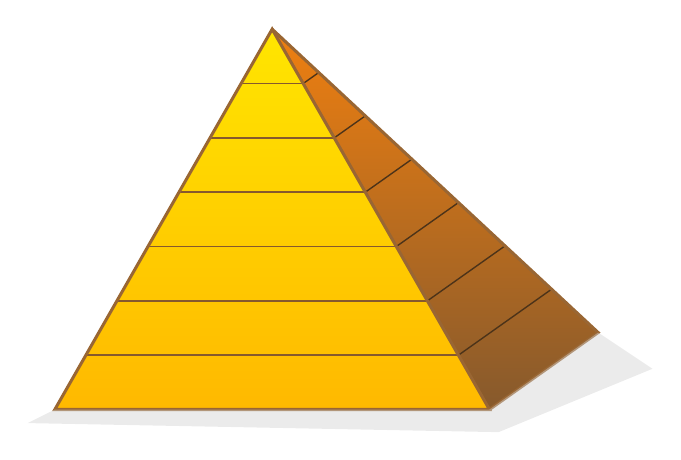
\begin{tikzpicture}[scale=1.15]
  % Front sunlit face of the pyramid
  \fill[top color=yellow!80!orange, bottom color=orange!55!yellow]
    (0,0) -- (4.8,0) -- (2.4,4.2) -- cycle;
  % Right shaded 3D face of the pyramid
  \fill[top color=orange!75!brown, bottom color=brown!70!black]
    (4.8,0) -- (6.0,0.85) -- (2.4,4.2) -- cycle;
  % Stone course horizontal lines on front face
  \foreach \k in {1,2,3,4,5,6} {
    \pgfmathsetmacro{\y}{0.6*\k}
    \pgfmathsetmacro{\xl}{2.4*(\y/4.2)}
    \pgfmathsetmacro{\xr}{4.8 - 2.4*(\y/4.2)}
    \draw[brown!70!black, line width=0.55pt] (\xl,\y) -- (\xr,\y);
    % Matching perspective lines on right shaded face
    \pgfmathsetmacro{\rx}{6.0 - (6.0-2.4)*(\y/4.2)}
    \pgfmathsetmacro{\ry}{0.85 + (4.2-0.85)*(\y/4.2)}
    \draw[brown!40!black, line width=0.5pt] (\xr,\y) -- (\rx,\ry);
  }
  % Outer edges
  \draw[brown!80!black, line width=1.1pt]
    (0,0) -- (4.8,0) -- (2.4,4.2) -- cycle;
  \draw[brown!80!black, line width=1.1pt]
    (4.8,0) -- (6.0,0.85) -- (2.4,4.2);
  % Ground shadow
  \fill[gray!35, opacity=0.45]
    (0,0) -- (4.8,0) -- (6.0,0.85) -- (6.6,0.45) -- (4.9,-0.25) -- (-0.3,-0.15) -- cycle;
\end{tikzpicture}

\vspace{14pt}
{\Huge\bfseries\color{brown!75!black}\begin{CJK}{UTF8}{bsmi}我成功了！\end{CJK}}
\end{center}
\vspace*{\fill}

\end{document}
